\section{Results}

In this section, we compare the results from Moltres for each benchmark step to
the results reported in the the benchmark paper \cite{tiberga_results_2020}.
The benchmark paper contains results from four different \gls{MSR} simulation
software packages. The authors of the benchmark performed code-to-code verification by reporting
the average discrepancy $\epsilon$ from all software packages for each
benchmark step. The discrepancy $\epsilon_c$ from each software package for
each measured quantity $Q_c$ calculated using the following equation:
%
\begin{align}
    \epsilon_c &= \sqrt{\frac{\sum^{N_p}_{i=1}\left(Q_c(\vec{r_i}) - Q_{avg}
    (\vec{r_i})\right)^2}{\sum^{N_p}_{i=1} Q^2_{avg}(\vec{r_i})}}
    \intertext{where}
    N_p &= 201 \nonumber \\
    &= \mbox{number of sampling points of quantity $Q$,}
    \nonumber \\
    N_c &= \mbox{number of \gls{MSR} software packages,} \nonumber \\
    Q_{avg}(\vec{r_i}) &= \frac{1}{N_c} \sum^{N_c}_{c=1} Q_c(\vec{r_i})
    \nonumber \\
    &= \mbox{average value of $Q$ at $\vec{r_i}$ from all packages.} \nonumber
\end{align}

\subsection{Phase 0 results \& discussion}

Table \ref{table:disc0} shows the discrepancy values from Moltres for Phase 0
and the corresponding average discrepancy values from the benchmark
\cite{tiberga_results_2020}. Moltres performs excellently as all discrepancy
values are within the same order of magnitude as those from the benchmark,
except the discrepancy value for $T$ along centerline BB'. We also observe in
table \ref{table:rho} that the $\rho$ value from Moltres falls within the
range of $\rho$ values from the benchmark.

Moltres reports a slightly larger discrepancy in the fission rate density as
we used zeroth-order shape functions to approximate the precursor
concentrations $C_i$. These shape functions perform worse in approximating
$C_i$ near the boundaries where the gradient is steeper in the homogeneous
domain with no reflectors.

The temperature values at the end of centerline BB', near the top boundary,
deviated significantly (912 K from Moltres
vs. ~935 K from the benchmark). The finite element method struggles with
the velocity boundary condition discontinuity on the top left corner of the
domain. As such, we observe the temperature deviation
directly downstream of the discontinuity.
%
\begin{table}[t!]
	\caption{Discrepancy values for the results from Phase 0.}
	\centering
	\small
	\setlength\tabcolsep{2.5pt}
	\begin{tabular}{l l l S S}
		\toprule
		\multirow{2}{*}{\textbf{Step}} & \multirow{2}{*}{\textbf{Observable}} & \multirow{2}{*}{\textbf{Source}} & \multicolumn{2}{c}{\textbf{Discrepancies [\%]}} \\
		& & & {Along AA'} & {Along BB'} \\
		\midrule
		\multirow{4}{*}{0.1} &
		\multirow{2}{*}{$u_x$ [m$\cdot$s$^{-1}$]} & Moltres & 0.247 & 0.266 \\
		& & Benchmark & 0.253 & 0.318 \\
		& \multirow{2}{*}{$u_y$ [m$\cdot$s$^{-1}$]} & Moltres & 0.540 & 0.467
		\\
		& & Benchmark & 0.598 & 0.795 \\
		\midrule
		\multirow{2}{*}{0.2} &
		\multirow{2}{*}{$\sum^G_i \Sigma_{f,i} \phi_i(\vec{r})$
		[m$^{-3}\cdot$s$^{-1}$]} & Moltres & 0.313 & {N.A.} \\
		& & Benchmark & 0.285 & {N.A.} \\
		\midrule
		\multirow{2}{*}{0.3} &
		\multirow{2}{*}{$T$ [K]} & Moltres & 0.090 & 0.164 \\
		& & Benchmark & 0.085 & 0.083 \\
		\bottomrule
	\end{tabular}
	\label{table:disc0}
\end{table}
%
\begin{table}[t!]
    \caption{Reactivity $\rho$ and change in reactivity
    $\left(\rho_a - \rho_b\right)$ values from Steps 0.2, 1.1,
    1.2, and 1.3. All units are in pcm.}
    \centering
    \small
    \setlength\tabcolsep{3.3pt}
    \begin{tabular}{l S S S S}
        \toprule
        \multirow{2}{*}{\textbf{Source}} & {\textbf{Step 0.2}} &
        {\textbf{Step 1.1}} & {\textbf{Step 1.2}} & {\textbf{Step 1.3}} \\
        & {$\rho_{s_{0.2}}$}
        & {$\rho_{s_{1.1}} - \rho_{s_{0.2}}$}
        & {$\rho_{s_{1.2}} - \rho_{s_{1.1}}$}
        & {$\rho_{s_{1.2}} - \rho_{s_{0.2}}$} \\
        \midrule
        Moltres     & 465.6 & -62.9 & -1142.2 & -1207.7 \\
        CNRS-$SP_1$ & 411.3 & -62.5 & -1152.0 & -1220.5 \\
        CNRS-$SP_3$ & 353.7 & -62.6 & -1152.7 & -1220.7 \\
        Polimi      & 421.2 & -62.0 & -1161.0 & -1227.0 \\
        PSI         & 411.7 & -63.0 & -1154.8 & -1219.6 \\
        TUD-$S_2$   & 482.6 & -62.0 & -1145.2 & -1208.5 \\
        TUD-$S_6$   & 578.1 & -60.7 & -1122.0 & -1184.4 \\
        \bottomrule
    \end{tabular}
    \label{table:rho}
\end{table}

\subsection{Phase 1 results \& discussion}

Figure \ref{fig:color} shows the typical temperature distribution and velocity
streamlines from running a fully coupled problem in Step 1.4. 
Table \ref{table:disc1} shows the discrepancy values from Moltres for Steps
1.1, 1.2, and 1.3,
and the corresponding average discrepancy values from the benchmark
\cite{tiberga_results_2020}. The subsequent subsections discuss the results
for each benchmark step.
%
\begin{figure}[H]
  \centering
  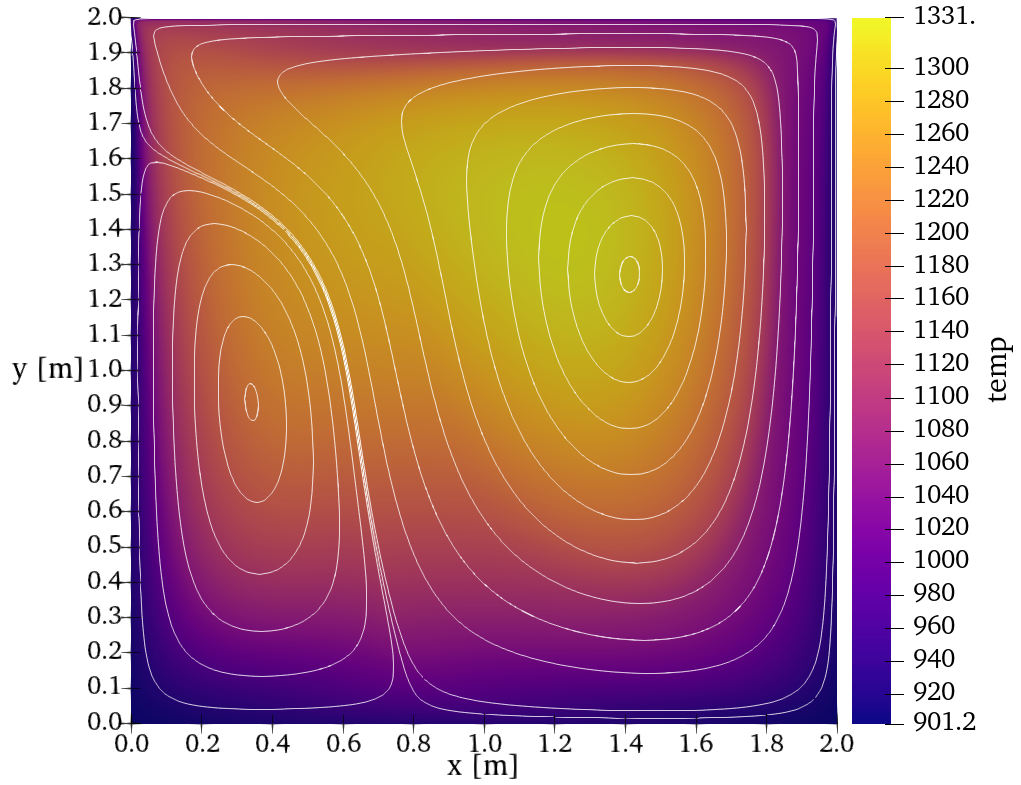
\includegraphics[width=\columnwidth]{full-coupled}
  \caption{The temperature distribution in the domain for the fully coupled
  system (Step 1.4) with buoyancy effects, $P = 1$ GW, and $U_{lid} = 0.5$
  m$\cdot$s$^{-1}$. The lines correspond to the streamlines of the velocity
  field.}
  \label{fig:color}
\end{figure}

\subsubsection{Step 1.1: Circulating fuel}

Moltres performs relatively worse than the benchmark average, but the
discrepancies are still on the same order of magnitude. We attribute this to
the same zeroth-order shape function approximation for the precursor
concentration mentioned in Step 0.2.

On the other hand, we observe in Table \ref{table:rho} that the change in
$\rho$ relative to Step 0.2 falls within the reported range of $\rho$ values
from the benchmark.

\begin{table}[htb!]
	\caption{Discrepancy values for the results from Phase 1.}
	\centering
	\small
	\setlength\tabcolsep{2.5pt}
	\begin{tabular}{l p{27mm} l S S}
		\toprule
		\multirow{2}{*}{\textbf{Step}} & \multirow{2}{*}{\textbf{Observable}} & \multirow{2}{*}{\textbf{Source}} & \multicolumn{2}{c}{\textbf{Discrepancies [\%]}} \\
		& & & {Along AA'} & {Along BB'} \\
		\midrule
		\multirow{2}{*}{1.1} &
		\multirow{2}{*}{$\sum_j \lambda_j C_j$ [m$^{-3}\cdot$s$^{-1}$]} & Moltres & 0.606 & 0.378 \\
		& & Benchmark & 0.346 & 0.294 \\
		\midrule
		\multirow{4}{*}{1.2} &
		\multirow{2}{*}{$T$ [K]} & Moltres & 0.076 & 0.179 \\
		& & Benchmark & 0.095 & 0.089 \\
		& {\footnotesize $\Delta\left[\sum^G_i \Sigma_{f,i} \phi_i(\vec{r})
		\right]_{s_{1.2}-s_{0.2}}$} & Moltres & 1.110 & 1.082 \\
		& {\footnotesize [m$^{-3}\cdot$s$^{-1}$]} & Benchmark & 1.576 & 1.133 \\
		\midrule
		\multirow{8}{*}{1.3} &
		\multirow{2}{*}{$u_x$ [m$\cdot$s$^{-1}$]} & Moltres & 0.123 & {N.A.} \\
		& & Benchmark & 0.691 & {N.A.} \\
		& \multirow{2}{*}{$u_y$ [m$\cdot$s$^{-1}$]} & Moltres & 0.236 & 0.238 \\
		& & Benchmark & 0.329 & 0.356 \\
		& \multirow{2}{*}{$T$ [K]} & Moltres & 0.064 & 0.070 \\
		& & Benchmark & 0.057 & 0.080 \\
		& \multirow{2}{*}{$\sum_j \lambda_j C_j$ [m$^{-3}\cdot$s$^{-1}$]} & Moltres & 1.079 & 0.5780 \\
		& & Benchmark & 0.460 & 1.194 \\
		\bottomrule
	\end{tabular}
	\label{table:disc1}
\end{table}

\subsubsection{Step 1.2: Power coupling}

For this step, Moltres performed better than the benchmark average except
the temperature distribution along BB', the cause of which we
addressed in Step 0.3. The smaller discrepancy in the change in fission rate
density indicates that Moltres is on average more self-consistent since this
quantity measures the difference between two sets of data from the same
software. From Table \ref{table:rho}, Moltres also reports a change in $\rho$,
relative to Step 1.1, that falls within the range of benchmark values.

\subsubsection{Step 1.3: Buoyancy}

Moltres performs reasonably well in Step 1.3, with smaller
discrepancies in most of the velocity components and temperature distribution
than the benchmark average. Moltres bucks the trend for discrepancies
in the delayed neutron source as the discrepancy along AA' is
noticeably worse than the benchmark average, but Moltres performs relatively
better along BB'. In Table \ref{table:rho}, we observe once again that the
change in $\rho$ in Moltres falls within the range of benchmark values.

\subsubsection{Step 1.4: Full coupling}

Table \ref{table:full} shows the change in $\rho$ under the various $U_{lid}$
and $P$ values. We refer readers to Tiberga et al.'s paper
\cite{tiberga_results_2020} for the benchmark's corresponding values.
The results from Moltres all fall within the range of benchmark values for all
cases. Furthermore, the $\Delta\rho$ values are all within 1.1 pcm of the
corresponding values from the TUD-S$_2$ model in the benchmark paper. Given
that the $S_2$ discrete ordinates method is qualitatively similar to the
multigroup neutron diffusion method, this shows that Moltres is
consistent to the benchmark within the limitations brought about by the neutron
diffusion method.

\begin{table}[htbp!]
	\caption{Reactivity change in Step 1.4, relative to Step 0.2 under various
	$U_{lid}$ and $P$ values.}
	\centering
	\small
	\setlength\tabcolsep{1.5pt}
	\begin{tabular}{c c c c c c}
		\toprule
		& \multicolumn{5}{c}{$\rho - \rho_{s0.2}$ [pcm]} \\
		\midrule
		{\backslashbox{$U_{lid}$ [m$\cdot$s$^{-1}$]}{$P$ [GW]}} & 0.2 & 0.4 & 0.6 & 0.8 & 1.0 \\
		\midrule
		0.0 & -263.7 & -498.3 & -730.9 & -966.7 & -1207.7 \\
		0.1 & -265.9 & -498.7 & -730.6 & -966.0 & -1206.7 \\
		0.2 & -268.1 & -498.8 & -729.4 & -963.7 & -1203.6 \\
		0.3 & -269.9 & -498.5 & -727.8 & -960.8 & -1199.5 \\
		0.4 & -271.9 & -498.5 & -726.5 & -958.3 & -1195.7 \\
		0.5 & -274.2 & -498.7 & -725.6 & -956.4 & -1192.7 \\
		\bottomrule
	\end{tabular}
	\label{table:full}
\end{table}
